\subsection{Squirmerモデル}
    \begin{figure}[htbp]
        \centering
        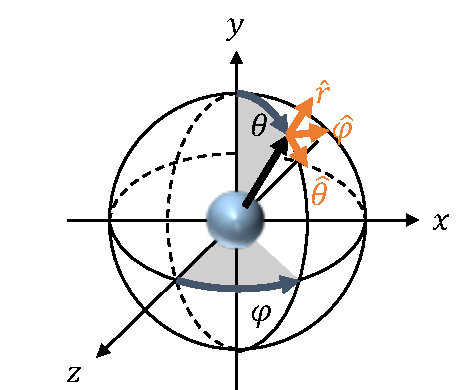
\includegraphics[scale=1.0]{/Users/taiga/Projects/lab/thesis/components/chapter2/figs/system.pdf}
        \caption{本実験の座標系}
        \label{fig:system}
    \end{figure}

マイクロスイマーのモデルとして,Squirmerモデル\cite{squirmer}を採用した.
このモデルでは,球形の粒子表面において,粒子と流体の速度差が式\eqref{eq:squirmer}で表されるようなsliding境界条件を用いる.

    \begin{equation}
        \boldsymbol{u}^\mathrm{s} = 
            \sum_{n=1}^\infty\frac{2}{n(n + 1)} B_n P_n^\prime(\cos{\theta}) \sin{\theta} \hat{\boldsymbol{\theta}}
        \label{eq:squirmer}
    \end{equation}

\noindent
ここで, 式中の$\theta$および$\boldsymbol{\hat{\theta}}$はFig.\ref{fig:system}のように表される角度および単位角度ベクトルである.
本研究では,$xy$平面上を$x$軸正の向きに流れるせん断流を考えたので,
Fig.\ref{fig:system}中の$\varphi$は$\pi / 2$で固定されているとした.
また,$\boldsymbol{u}^\mathrm{s}$はマイクロスイマー表面の重心に対するslide速度,
$B_n$は係数,
$P^\prime_n$は $n$次Legendre多項式の導関数である.
しかし,$n=1$の項はsquirmerの泳動速度を,
$n=2$の項はsquirmerの存在によって生じる応力を決めるが,
$n \geq 3$の項は,泳動速度,および応力に影響を与えないので,
式\eqref{eq:squirmer}は,第1,2項のみを考えることで,式\eqref{eq:squirmer2}の様に簡略化できる.

    \begin{equation}
        \boldsymbol{u}^s =
            B_1 \left( \sin{\theta} + \frac{\alpha}{2} \sin{2\theta} \right) \hat{\boldsymbol{\theta}}
        \label{eq:squirmer2}
    \end{equation}

\noindent
ここで,$B_1$はマイクロスイマーの進行速度の大きさ$(U = 2/3 B_1)$を与える.
ただし,本研究では,squirmer粒子の移動の影響を排除するために,$B_1 = 0.01$と十分に小さい値に設定した.
また,$\alpha = B_2/B_1$はその符号によりスイマーの種類を表す定数となる.
$\alpha > 0$をPuller型,$\alpha = 0$をNeutral型,$\alpha < 0$をPusher型と呼ぶ.
Puller型は,周辺流体に収縮流を生成し,Pusher型は伸長流を生成する.

    \begin{figure}[H]
        \centering
        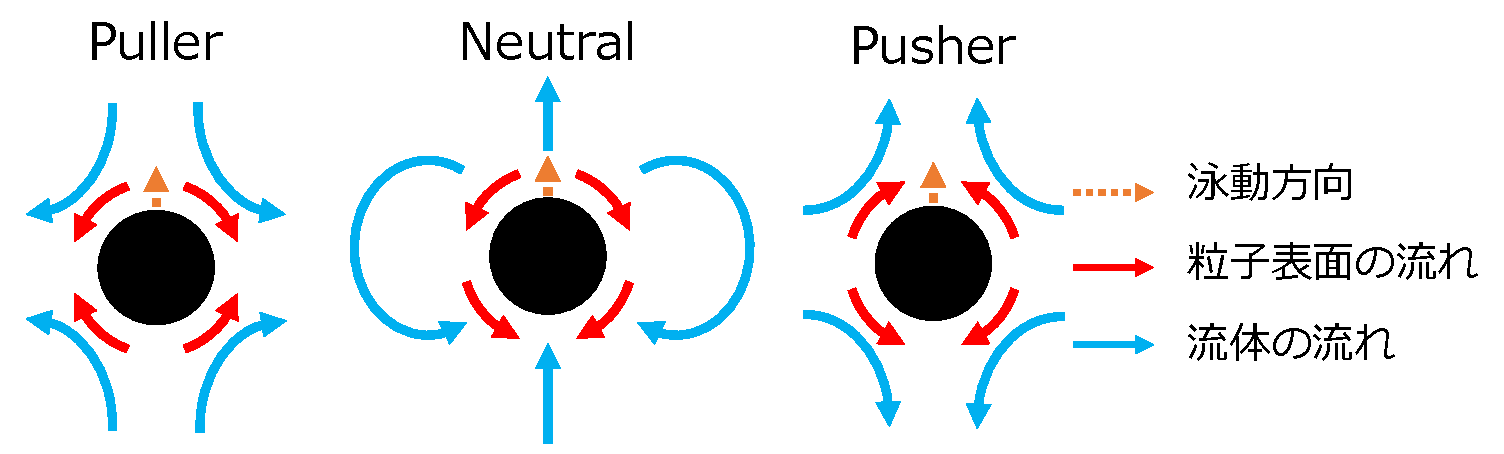
\includegraphics[scale=0.5]{/Users/taiga/Projects/lab/thesis/components/chapter2/figs/microswimmers.pdf}
        \caption{SquirmerモデルにおけるPusher型,Neutral型,Puller型の概略図}
        \label{fig:squirmermodel}
    \end{figure}
